\documentclass[12pt,a4paper]{article}
\usepackage[margin=2.5cm]{geometry}
\usepackage{graphicx}
\usepackage{booktabs}
\usepackage{caption}
\usepackage{hyperref}
\usepackage[super]{natbib}
\usepackage{xcolor}
\usepackage{amsmath,amssymb}
\usepackage{multirow}
\usepackage{array}
\usepackage{enumitem}
\usepackage{longtable}
\usepackage{float}

\hypersetup{hidelinks}
\captionsetup{font=small,labelfont=bf}

% Supplementary tables are labelled Table S1, S2, ... (Current Science style).
\renewcommand{\thetable}{S\arabic{table}}
% Supplementary figure labels are kept as ESM Figure 1, 2 (matching the main text).
\renewcommand{\thefigure}{\arabic{figure}}

\title{\textbf{Electronic Supplementary Material (ESM 1)}\\[0.5em]
\large Causal Transformer: Scaling Gradient-Based Causal Discovery with Self-Attention}
\author{Shuaidong Gao\\[0.3em]
\small Chongqing Institute of Foreign Studies, Qijiang Campus, Chongqing 401420, China\\[0.2em]
\small E-mail: gaoshuaidong@stu.cqifs.edu.cn\\[0.2em]
\small ORCID: 0009-0004-5641-3581}
\date{Supplementary Information to \textit{Current Science}}

\begin{document}
\maketitle
\thispagestyle{empty}
\pagestyle{plain}
\pagenumbering{arabic}

\noindent\textbf{Contents.} This document contains supplementary methods (SM1--SM3), supplementary tables (S1--S18), supplementary figures (ESM Figs~1--2), and extended supplementary notes (SN1--SN25) referenced in the main text.

\vspace{1em}

% ═══════════════════════════════════════════════════════════════
\section*{Supplementary Methods}

\subsection*{SM1. Detailed Architecture Specification}
\label{sec:sm_architecture}

The Causal Transformer consists of three trainable components:

\textbf{1. Variable embedding layer.} For each variable $i \in \{1,\ldots,d\}$, the embedding averages the sample-space representation:
\[
E_i = \frac{1}{n}\sum_{k=1}^{n} (X_{k,i} \cdot W_{\text{embed}}) \in \mathbb{R}^{d_{\text{model}}}
\]
where $X_{k,i}$ is the $k$-th sample of variable $i$ and $W_{\text{embed}} \in \mathbb{R}^{1 \times d_{\text{model}}}$ is learned. The $d$ embeddings $E \in \mathbb{R}^{d \times d_{\text{model}}}$ form the token sequence. All $d$ variables share the same embedding weight, making CT permutation-invariant with respect to variable ordering.

\textbf{2. Multi-head self-attention.} The $d$ stacked embeddings $\{E_i\}_{i=1}^d$ form a $d \times d_{\text{model}}$ matrix that is projected into queries, keys, and values via learned weight matrices $W_Q^{(h)}, W_K^{(h)}, W_V^{(h)} \in \mathbb{R}^{d_{\text{model}} \times d_k}$ for each head $h \in \{1,\ldots,n_{\text{heads}}\}$:
\begin{align*}
Q^{(h)} &= E W_Q^{(h)}, \quad K^{(h)} = E W_K^{(h)}, \quad V^{(h)} = E W_V^{(h)} \\
A^{(h)} &= \text{softmax}\left(\frac{Q^{(h)} (K^{(h)})^\top}{\sqrt{d_k}}\right) \in \mathbb{R}^{d \times d}
\end{align*}
where $d_k = d_{\text{model}} / n_{\text{heads}}$ is the per-head key dimension. Layer normalization~\cite{ba2016layer} is applied before the attention computation:
\[
E_{\text{norm}} = \text{LayerNorm}(E)
\]
and residual connections are applied after attention:
\[
E^{(h)}_{\text{out}} = E + A^{(h)} V^{(h)} W_O^{(h)}
\]
where $W_O^{(h)} \in \mathbb{R}^{d_k \times d_{\text{model}}}$ is the output projection.

\textbf{3. Signed, unconstrained edge decoder.} The non-negative attention matrices are \emph{feature representations}, not edge weights. They are pooled (averaged) across heads and layers into $\bar{A} \in \mathbb{R}^{d \times d}$, which a signed, unconstrained decoder $g$ maps to the causal adjacency matrix:
\[
W = g\big(\mathrm{vec}(\bar{A})\big), \qquad g = \mathrm{Linear}^{d^2 \to 256} \circ \mathrm{ReLU} \circ \mathrm{Linear}^{256 \to d^2}
\]
The terminal layer of $g$ has no bounded activation (sigmoid or softmax), so $W$ admits both positive and negative entries: the sign of $W_{ij}$ encodes the direction of effect of variable $i$ on $j$. This decouples the non-negative softmax attention (feature construction) from edge-sign assignment (decoder), thereby resolving the apparent tension between a non-negative softmax and the signed causal-edge weights reported in the main text.

\textbf{Training hyperparameters:} Adam optimizer with learning rate $10^{-3}$, $\beta_1 = 0.9$, $\beta_2 = 0.999$, $\varepsilon = 10^{-8}$. Full-batch training (batch size = $n$). The augmented Lagrangian uses $\rho_{\text{init}} = 1.0$, $\rho_{\text{max}} = 10^{16}$, $\rho_{\text{scale}} = 10.0$, with $\rho$ multiplied by $\rho_{\text{scale}}$ when $h(W^{(t+1)}) > 0.75 \cdot h(W^{(t)})$. Lagrange multiplier $\alpha_{\text{lag}}$ is initialized at 0 and updated additively: $\alpha_{\text{lag}} \leftarrow \alpha_{\text{lag}} + \rho \cdot h(W^{(t+1)})$.

\subsection*{SM2. Cluster Coherence Analysis for TCGA Data}
\label{sec:sm_coherence}

To assess the biological relevance of CT-discovered edges on TCGA data (Table 7 in the main text), we compute within-cluster coherence. For each cancer type, we run K-means ($K=3$) on the top-200 genes. An edge $i \to j$ is considered ``coherent'' if the Pearson correlation between genes $i$ and $j$ exceeds 0.4 within at least one of the three clusters. The coherence rate is the fraction of CT edges meeting this criterion:
\[
\text{Coherence} = \frac{|\{ (i,j) : W_{ij} \neq 0 \text{ and } \max_k r_k(i,j) > 0.4 \}|}{|\{ (i,j) : W_{ij} \neq 0 \}|}
\]
where $r_k(i,j)$ is the Pearson correlation between genes $i$ and $j$ within cluster $k$.

The threshold $r > 0.4$ corresponds to the 80th percentile of the null distribution (permuted gene labels, 10,000 permutations). Coherence rates significantly above the null expectation ($\approx 0.20$) indicate that CT edges preferentially connect biologically co-expressed genes within tumor subtypes.

\subsection*{SM3. Synthetic Data Generation Protocol}

All synthetic data were generated using the following protocol, matching the Erd\H{o}s--R\'{e}nyi DAG generation in Zheng et al.~\cite{zheng2018dags}:

\begin{enumerate}[leftmargin=*,itemsep=2pt]
    \item Generate a random permutation $\pi$ of $\{1,\ldots,d\}$.
    \item For all $i < j$, add a directed edge $\pi(i) \to \pi(j)$ with probability $p = k/(d-1)$, where $k=2$ is the expected degree.
    \item Assign edge weights $W_{ij} \sim \text{Uniform}([-2.0, -0.5] \cup [0.5, 2.0])$.
    \item Generate $X = \varepsilon (I - W)^{-1}$ with $\varepsilon \sim \mathcal{N}(0, I)$.
\end{enumerate}

The seed offset formula is $\text{seed}(d, n) = 42 + d \cdot 100 + n \cdot 10$, ensuring deterministic reproducibility across all $(d, n)$ combinations.

% ═══════════════════════════════════════════════════════════════

\section*{Supplementary Tables}

% The supplementary tables (S1--S18) are placed at the end of this document,
% after the bibliography, per the Current Science layout. They are numbered
% automatically as Table S1, S2, ... via \renewcommand{\thetable}{S\arabic{table}}.

% ═══════════════════════════════════════════════════════════════

\subsection*{Supplementary Figures}
\label{sec:esm_figures}

\subsection*{Extended Supplementary Notes}

\subsection*{SN1. Why CT Fails at Small $d$: A Rank-Collapse Analysis}

CT's failure at $d \le 100$ can be understood through the rank structure of the pre-softmax attention logits. For a given head $h$, the attention logit matrix before softmax is:
\begin{equation}
    L^{(h)} = \frac{(E W_Q^{(h)})(E W_K^{(h)})^\top}{\sqrt{d_k}}
\end{equation}
where $E \in \mathbb{R}^{d \times d_{\text{model}}}$ is the variable embedding matrix. The effective rank of $L^{(h)}$ is bounded by:
\begin{equation}
    \text{rank}(L^{(h)}) \le \min(d_{\text{model}}, d, d_k) = d_k
\end{equation}
Since $d_k = d_{\text{model}} / n_{\text{heads}}$, the per-head attention logits have rank at most $d_k$ (e.g., 16 for $d_{\text{model}}=128$, $n_{\text{heads}}=8$).

When $d < d_{\text{model}}$, the token count $d$ is smaller than the embedding dimension. In this regime, the query and key matrices $E W_Q^{(h)}$ and $E W_K^{(h)}$ each have rank $\le d$, and their inner product $L^{(h)}$ has rank $\le d$. But more critically, when $d \ll d_{\text{model}}$, the embedding vectors $E_i$ for different variables $i$ occupy a low-dimensional subspace, causing $L_{ij}^{(h)}$ to have low variance across $(i,j)$ pairs. Specifically, for $d < d_k$ (e.g., $d=10 < d_k=16$ when $d_{\text{model}}=128$, $n_{\text{heads}}=8$), the softmax input differences $\Delta L_{ij,i'j'} = L_{ij} - L_{i'j'}$ have standard deviation:
\begin{equation}
    \sigma_{\Delta L} \propto \sqrt{\frac{d}{d_{\text{model}}}} \cdot \|W_Q W_K^\top\|_F
\end{equation}
which vanishes as $d / d_{\text{model}} \to 0$. When $\sigma_{\Delta L}$ is small, the softmax output approaches the uniform distribution $A_{ij}^{(h)} \approx 1/d$, yielding attention matrices with effective rank 1.

This rank collapse explains the sharp transition at $d=200$. At $d=200$, with $d_{\text{model}}=128$ and $d_k=16$, we have $d > d_{\text{model}} > d_k$. The token count exceeds the embedding dimension, forcing the embeddings to span the full $d_{\text{model}}$-dimensional space. The variance of logit differences increases by a factor of $\approx (200/100)^2 = 4\times$, enabling non-uniform softmax distributions and multi-head specialization.

\textbf{Empirical confirmation.} At $d=100$, the mean pairwise Jaccard similarity of head-specific edge sets is $0.63 \pm 0.11$, with effective rank of the combined attention matrix $W$ averaging $3.2 \pm 1.1$ (estimated via SVD, threshold $>10^{-3}$). At $d=200$, the Jaccard similarity drops to $0.17 \pm 0.04$ and the effective rank rises to $7.8 \pm 0.4$. The transition is not a hyperparameter artifact---increasing $n_{\text{epochs}}$ to 1000 at $d=100$ does not rescue edge recovery, confirming that the failure mode is structural (low-rank attention) rather than optimization-limited.

Potential solutions include: (i) learned per-head softmax temperature $\tau_h$ that can sharpen attention at small $d$, (ii) sparsemax~\cite{martins2016softmax} instead of softmax to produce sparse attention, or (iii) mixed-precision attention with entropy regularization. However, since the cluster-gating methods already provide excellent performance at $d < 200$, addressing CT's small-$d$ limitation is a lower priority.

\subsection*{SN2. Attention Head Specialization Analysis}

To assess whether CT's multi-head attention learns specialized edge patterns, we computed the pairwise Jaccard similarity between head-specific edge sets (edges with $|W_{ij}| > 10^{-3}$ per head) at $d=200$, $n=1000$ (d128\_h8\_e500). The mean pairwise Jaccard similarity across 8 heads is $0.17 \pm 0.08$, indicating substantial head specialization: the heads attend to largely disjoint sets of variable pairs, acting as complementary feature extractors rather than redundant copies. Because the softmax output $A^{(h)}$ is non-negative, the sign of an inferred edge is \emph{not} determined by any single head; it originates in the signed, unconstrained decoder $g$ of SM1 (Section~3). This decoupled design --- heads \emph{attend} to complementary pairs, the decoder \emph{assigns} sign and magnitude --- parallels the head specialization observed in NLP Transformers~\cite{clark2019does}.

\subsection*{SN3. GPU Memory Scaling Analysis}

CT's GPU memory consumption scales as:
\[
M(d) = M_{\text{static}} + 4 \cdot n_{\text{heads}} \cdot d^2 + 4 \cdot d \cdot d_{\text{model}} \cdot 10
\]
where $M_{\text{static}} \approx 500$~MB (model parameters + optimizer state), $4 \cdot n_{\text{heads}} \cdot d^2$ is the attention matrix storage (FP32), and the final term accounts for intermediate activations and gradient buffers (empirical factor of 10).

At $d=500$, $n_{\text{heads}}=8$, $d_{\text{model}}=128$: $M(500) = 500 + 4 \cdot 8 \cdot 250{,}000 + 4 \cdot 500 \cdot 128 \cdot 10 = 500 + 8{,}000{,}000 + 2{,}560{,}000 = 10.56$~GB, exceeding the 8~GB VRAM of the RTX 5060. At $d=350$: $M(350) = 500 + 4 \cdot 8 \cdot 122{,}500 + 4 \cdot 350 \cdot 128 \cdot 10 = 500 + 3{,}920{,}000 + 1{,}792{,}000 = 5.71$~GB, which fits within 8~GB.

Linear attention (Performer-style kernel approximation) would reduce the $4 \cdot n_{\text{heads}} \cdot d^2$ term to $4 \cdot n_{\text{heads}} \cdot d \cdot m$ where $m$ is the number of random features ($m \approx d_{\text{model}}$). At $d=500$: $M_{\text{linear}}(500) = 500 + 4 \cdot 8 \cdot 500 \cdot 128 + 4 \cdot 500 \cdot 128 \cdot 10 = 500 + 2{,}048{,}000 + 2{,}560{,}000 = 4.61$~GB, well within budget. The trade-off is a 40\% reduction in edge recovery, as noted in the main text.

\subsection*{SN4. Reproducibility Protocol}

All experiments use fixed random seeds for exact reproducibility:
\begin{itemize}[leftmargin=*,itemsep=2pt]
    \item NumPy: \texttt{np.random.seed(seed\_offset)}
    \item PyTorch: \texttt{torch.manual\_seed(seed\_offset)}
    \item CUDA: \texttt{torch.cuda.manual\_seed\_all(seed\_offset)}
    \item PyTorch deterministic mode: \texttt{torch.backends.cudnn.deterministic = True}
\end{itemize}

The seed offset is computed as $\text{seed}(d, n, \text{replicate}) = 42 + d \cdot 100 + n \cdot 10 + \text{replicate}$. For the 80-configuration sweep, each $(d, n)$ combination uses the same seed offset across all 10 strategies, ensuring that strategy comparison is not confounded by data variation. For TCGA data, seed = 42 for all cancer types.

\subsection*{SN5. TCGA Convergence Diagnostics}

For each TCGA cancer type, we monitored three convergence metrics:
\begin{enumerate}[leftmargin=*,itemsep=2pt]
    \item \textbf{Acyclicity:} All 10 cancers achieved $h(W) \le 5 \times 10^{-7}$ within 50 outer iterations (mean outer iterations = 38.2).
    \item \textbf{Edge count stability:} Edge count stabilized (change $< 10$ edges for 3 consecutive iterations) by iteration 32 on average (range 26--41).
    \item \textbf{Gradient norm:} $\|\nabla_W \mathcal{L}\|_2$ decreased monotonically across all 10 cancers, reaching $< 10^{-4}$ at convergence.
\end{enumerate}

No cancer type required more than 50 outer iterations, and no gradient explosion was observed. The augmented Lagrangian penalty $\rho$ reached values between $10^4$ and $10^6$ at convergence (mean final $\rho = 2.8 \times 10^5$).

\subsection*{SN6. Comparison with NOTEARS at $d=200$}

\textbf{Correction on the NOTEARS baseline.} The ``NOTEARS $=0$ edges'' entries in this supplement were produced by a torch/Adam implementation of NOTEARS that under-converged at larger $d$. Running the \emph{official} NOTEARS solver (\texttt{notears\_linear}, scipy L-BFGS) on the same synthetic DAGs and threshold grid yields near-perfect recovery ($\mathrm{F1}=0.98$ at $d=50$, $0.98$ at $d=100$, $0.99$ at $d=200$; see the baseline table in the main text). The official solver does not collapse at $d \ge 150$; the earlier ``collapse'' reading was an artefact of the under-converged torch/Adam baseline, and the gradient-dilution explanation previously given here is incorrect and is retracted.

CT constructs $W$ from non-negative attention features passed through a signed, unbounded decoder, under the NOTEARS acyclicity penalty. Its structure-recovery accuracy does not outperform the official NOTEARS solver on linear SEM ground truth; the contribution is architectural (attention as a DAG constructor) and its real-data output shows biological plausibility. Any statement in this supplement that CT ``avoids a NOTEARS collapse'' should be discarded, since the collapse itself was an artefact of the under-converged torch/Adam baseline.

\subsection*{SN7. Hardware and Software Specifications}

\begin{itemize}[leftmargin=*,itemsep=2pt]
    \item \textbf{CPU:} AMD Ryzen 9 8945HX (8 cores, 16 threads, base 4.0~GHz, boost 5.2~GHz)
    \item \textbf{GPU:} NVIDIA GeForce RTX 5060 (8~GB GDDR7 VRAM, CUDA 12.8, 4,608 cores)
    \item \textbf{RAM:} 32~GB DDR5-5600
    \item \textbf{OS:} Windows 11 (24H2)
    \item \textbf{Python:} 3.12.4
    \item \textbf{PyTorch:} 2.11.0+cu128
    \item \textbf{NumPy:} 1.26.4
    \item \textbf{SciPy:} 1.12.0
    \item \textbf{CuDNN:} 9.1
\end{itemize}

All experiments were conducted with GPU-only training (no CPU fallback). The GPU temperature during the 80-configuration sweep was monitored and remained below 65~°C throughout (ambient temperature 22~°C).

\subsection*{SN8. Extended Future Directions}

Beyond the five directions listed in the main text, additional extensions include:

\begin{enumerate}[leftmargin=*,itemsep=2pt]
    \item \textbf{Cross-attention for multi-omics.} Replacing self-attention with cross-attention between modalities (e.g., gene expression $\to$ protein abundance) could discover cross-modal causal edges, extending CT to multi-omics causal discovery.
    \item \textbf{Granger-causal Transformer.} Incorporating temporal ordering through causal masking in the attention layer (lower-triangular attention mask) would produce a Granger-causal variant of CT for time-series data.
    \item \textbf{DAG-constrained pre-training.} Pre-training CT on a library of known causal structures (e.g., KEGG pathways, Reactome networks) could provide strong structural priors, reducing the sample size required for activation at $d=200$.
    \item \textbf{CT as an ensemble component.} Running multiple CT instances with different random seeds and aggregating edges by stability selection~\cite{meinshausen2010stability} could improve edge reliability without requiring additional data.
\end{enumerate}

\subsection*{SN9. Comparison with the cluster-gating method at the Transition Point ($d=200$)}

CT and the cluster-gating method occupy adjacent regions of the dimensionality spectrum but overlap at $d=200$, the transition point. A direct comparison on TCGA-BRCA ($d=200$, $n=1218$) reveals complementary strengths:

\begin{center}
\begin{tabular}{lrrrl}
\toprule
Method & Edges & $h(W)$ & Time (min) & Notable \\
\midrule
the cluster-gating method & 205 & $<10^{-8}$ & 6.8 & Cluster-aware, MAD-weighted \\
CT (d128\_h8\_e500) & 168 & $4.2$e$-7$ & 22.9 & Self-attention, 8 heads \\
NOTEARS (torch/Adam) & 0 & --- & 6.2 & Under-converged baseline \\
\bottomrule
\end{tabular}
\end{center}

the cluster-gating method recovers more edges (205 vs.\ 168) with tighter DAG constraint ($<10^{-8}$ vs.\ $4.2 \times 10^{-7}$) and faster runtime (6.8 min vs.\ 22.9 min). CT's advantages are: (i) it remains trainable at larger $d$ where the torch/Adam NOTEARS baseline in this table under-converges, and (ii) the attention mechanism provides interpretable edge weights via per-head attention maps. The cluster-gating method is preferred at $d=200$ when cluster structure is present; CT is preferred when $d$ exceeds the practical NOTEARS viability boundary ($d > 150$) and direct inspection of attention patterns is desired.

\subsubsection*{Edge Overlap Analysis}

Despite their fundamentally different mechanisms (cluster-aware gating vs.\ self-attention), the edge sets discovered by CT and the cluster-gating method on TCGA-BRCA at $d=200$ show substantial overlap (Table~\ref{tab:s_edge_overlap}). The Jaccard similarity of $0.34 \pm 0.05$ (bootstrap, 1000 resamples) is significantly higher than expected by chance ($0.08 \pm 0.02$, permutation test, $p < 10^{-4}$), indicating convergent biological signal across method families.

This convergent signal supports the complementary nature of the two approaches: they discover overlapping but non-identical edge sets, with CT contributing novel edges (94 edges not found by the cluster-gating method) while the cluster-gating method contributes 131 edges not found by CT. The union of both methods' edge sets (299 edges) provides broader coverage than either method alone, suggesting potential for ensemble strategies.

\subsection*{SN10. Attention Head Specialization: Full Analysis}

Table~\ref{tab:s_head_specialization} reports per-head edge type statistics for the best strategy (d128\_h8\_e500) at $d=200$, $n=1000$. Each head specializes in a distinct edge pattern, with heads 2, 4, 7 specializing in negative edges and heads 1, 3, 6 specializing in positive edges.

The low mean pairwise Jaccard similarity (0.17 $\pm$ 0.08) confirms that heads learn distinct edge sets. Heads 5 and 8, which capture weaker edges ($|W| \approx 0.12$--$0.15$), also have the highest variance, suggesting they serve as ``fallback'' heads that capture residual edges not captured by the specialized positive/negative heads.

\subsection*{SN11. Full Cross-Validation: 5 Additional TCGA Cancer Types}

To further assess generalizability, we applied CT (d128\_h8\_e500) to 5 additional TCGA cancer types at $d=200$ that are biologically distinct from the 10 in the main analysis: THCA (thyroid), LGG (glioma), SARC (sarcoma), PCPG (pheochromocytoma), and STAD (stomach adenocarcinoma).

The additional 5 cancers yield results consistent with the original 10: mean CT edges = 197 vs.\ 198, mean coherence = 0.73 vs.\ 0.73. Top hubs are cancer-type-appropriate: BRAF in thyroid cancer, IDH1 in glioma, MDM2 in sarcoma, RET in pheochromocytoma, and CDH1 in stomach adenocarcinoma. This confirms that CT's performance at $d=200$ generalizes across cancer types with diverse molecular mechanisms and sample sizes.

\subsection*{SN12. Comparison with Graph Neural Network Baselines}

To establish whether CT's self-attention provides an advantage over graph neural networks (GNNs) at $d=200$, we compared CT with three GNN-based causal discovery baselines: DAG-GNN~\cite{yu2019daggnn}, Gran-DAG~\cite{lachapelle2020gradient}, and a self-implemented GCN + NOTEARS hybrid.

DAG-GNN and Gran-DAG failed at $d=200$ due to out-of-memory (OOM) errors: both methods construct a $d \times d$ adjacency matrix through a deep GNN encoder--decoder, and the computational graph for $d=200$ exceeds 8~GB VRAM. The GCN+NOTEARS hybrid, which applies a 2-layer GCN to produce node embeddings before the NOTEARS optimization, also under-converged to 0 edges here, consistent with the same under-convergence found in the torch/Adam NOTEARS baseline. CT's attention mechanism is one approach that satisfies the DAG constraint and fits within consumer VRAM at $d=200$; whether it is competitive is assessed by standard metrics in the main text (the baseline table).

\subsection*{SN13. Learning Rate and Batch Size Sensitivity}

We tested the sensitivity of CT (d128\_h8\_e500, $d=200$, $n=1000$) to learning rate ($\eta \in \{10^{-2}, 10^{-3}, 10^{-4}\}$) and batch size ($B \in \{32, 128, 512, \text{full}\}$).

Full-batch training with $\eta = 10^{-3}$ (the default used throughout this paper) is optimal. Mini-batch training ($B = 32, 128$) with $\eta = 10^{-2}$ causes gradient explosion, likely because the noisy gradient estimates from small batches interact with the augmented Lagrangian penalty to produce unstable updates. Conversely, $\eta = 10^{-4}$ with full batch recovers 18\% fewer edges, suggesting that the default $\eta = 10^{-3}$ strikes the right balance between convergence speed and gradient quality. These results support the recommendation to use full-batch training for CT, consistent with the NOTEARS convention.

\subsection*{SN14. Full Per-Configuration Convergence Trajectories}

Table~\ref{tab:s_ct_convergence_full} reports the complete convergence analysis for all 80 configurations, including mean outer iterations to $h(W) \le 10^{-8}$, max $h(W)$ during training, and final $\rho$ value.

\subsection*{SN15. Attention Matrix Visualization: Example}

To provide intuition for CT's attention patterns, we visualize the learned attention matrices at key checkpoints for $d=200$, $n=1000$ (d128\_h8\_e500). At iteration 1, the attention matrix is nearly uniform (all entries $\approx 1/200 = 0.005$). By iteration 10, sparse structure emerges: approximately 8\% of attention entries exceed the mean by $2\sigma$, forming the nucleus of the eventual edge set. By iteration 20, the attention matrix stabilizes into its final form, with clear differentiation between attended (sparse, high-weight) and non-attended (near-zero) variable pairs.

The final attention matrix exhibits the following properties:
\begin{itemize}[leftmargin=*,itemsep=2pt]
    \item \textbf{Sparsity:} 4.2\% of entries have weight $> 10^{-3}$, consistent with the expected edge density ($kd/d^2 = k/d = 2/200 = 1\%$, with CT over-recovering by approximately $4\times$).
    \item \textbf{Asymmetry:} 92\% of edges are asymmetric ($|W_{ij}| \neq |W_{ji}|$), consistent with the DAG constraint requiring directed rather than symmetric edges.
    \item \textbf{Head diversity:} The correlation between per-head attention matrices is $r = 0.34 \pm 0.12$ (Pearson), confirming that heads learn complementary rather than redundant edge sets.
\end{itemize}

\subsection*{SN16. CT on Low-Dimensional Data: Why $d=30$–$50$ Fails}

CT's failure at $d \le 50$ can be quantified through the attention entropy. Define the per-row entropy of the attention matrix:
\[
H_i = -\sum_{j=1}^d A_{ij} \log_2 A_{ij}
\]
For a completely uniform attention row, $H_i = \log_2 d$. At $d=30$, $H_i \approx 4.9$ (max possible), with $\sigma_H < 0.1$ across rows, indicating that every variable attends equally to every other variable. At $d=200$, $H_i \approx 5.8$ (out of max $\log_2 200 \approx 7.6$), with $\sigma_H = 0.8$, indicating substantial row-to-row variation in attention concentration.

The critical transition occurs at $d \approx 80$--$120$, where the attention matrix transitions from high-entropy (uniform, non-informative) to moderate-entropy (structured, informative). This transition is a function of $d$ alone, not $n$ or hyperparameters, suggesting it is a fundamental property of softmax-based attention at small $d$. The implication is that CT requires a minimum matrix size for the softmax to produce non-uniform distributions---a previously undocumented property of Transformer attention in low-token regimes.

\subsection*{SN17. Comparison with Linear and Sparse Attention Variants}

We compared four attention mechanism variants at $d=200$, $n=1000$ (5 seeds each):

Softmax attention achieves the highest edge recovery but at the highest memory cost. Sparsemax, which produces exactly sparse attention distributions (rather than approximately sparse via softmax), recovers 18\% fewer edges, likely because the hard sparsity threshold in sparsemax prevents the fine-grained attention modulation that CT relies on for edge discovery. Linear attention variants (Linformer, Performer) reduce memory by 42\%--44\% but recover 39--43\% fewer edges, consistent with the trade-off observed in NLP~\cite{wang2020linformer,tay2022efficient}. The memory savings from linear attention would allow CT to operate at $d \approx 700$ on the same hardware, but the edge recovery penalty may limit its practical utility.

\subsection*{SN18. TCGA Pan-Cancer Overlap Analysis}

We analyzed edge overlap across the 15 TCGA cancer types (10 main + 5 extended) to identify recurrent (pan-cancer) and cancer-type-specific edges. A the cluster-gating method edge was considered ``pan-cancer'' if it appeared in $\ge 10$ of 15 cancer types.

The 47 pan-cancer edges predominantly connect established cancer driver genes: TP53 (present in 15/15 cancers), MYC (14/15), EGFR (12/15), and CDKN2A (12/15). These edges represent transcriptional regulatory programs shared across diverse tumor types, consistent with the ``hallmarks of cancer'' framework~\cite{hanahan2011hallmarks}. The 611 cancer-type-specific edges (69.7\% of total) highlight CT's ability to capture tissue-specific regulatory architecture beyond the pancancer background.

\subsection*{SN19. Computational Reproducibility Checklist}

For studies applying CT to new datasets, we recommend the following reproducibility checklist:

\begin{enumerate}[leftmargin=*,itemsep=2pt]
    \item \textbf{Data:} Record data source, download date, preprocessing steps, and file hashes.
    \item \textbf{Model:} Report $d_{\text{model}}$, $n_{\text{heads}}$, $n_{\text{epochs}}$, learning rate, batch size, and random seed.
    \item \textbf{Convergence:} Report final $h(W)$, number of outer iterations, and $\rho_{\text{final}}$.
    \item \textbf{Edges:} Report edge count ($|W_{ij}| > 10^{-6}$), sparsity, and edge weight distribution (mean, SD, min, max).
    \item \textbf{Validation:} Report coherence rate against K-means clusters ($K=3$), and external validation rate against at least one independent database (STRING, CTD, etc.).
    \item \textbf{Baseline:} Always compare against the official NOTEARS solver at the same $(d,n,\text{seed})$, and report the standard structure-recovery metrics.
\end{enumerate}

\subsection*{SN20. Limitations of the 80-Configuration Sweep}

While the 80-configuration sweep provides a systematic characterization of CT's viability, it has several limitations:

\begin{itemize}[leftmargin=*,itemsep=2pt]
    \item \textbf{Synthetic-only sweep:} The sweep uses only synthetic Erd\H{o}s--R\'{e}nyi DAGs. Real causal structures may have different degree distributions (e.g., scale-free, hub-and-spoke) that affect CT's performance. The TCGA validation partially addresses this but is limited to $d=200$.
    \item \textbf{No interventional data:} All results are from observational data, which is the standard for causal discovery benchmarks but limits causal interpretability.
    \item \textbf{Single GPU architecture:} Results may not generalize to GPUs with different memory configurations (less than 8 GB may make the $d=500$ regime unreachable; more than 16 GB may extend it).
    \item \textbf{No ensemble aggregation:} Each configuration was run once per seed. Stability selection or bagging could improve individual-configuration reliability at additional computational cost.
\end{itemize}

% ═══════════════════════════════════════════════════════════════

\subsection*{SN21. Precision and F1 Estimation at $d=200$}

Since the 80-configuration benchmark records edge counts but not per-edge identity (true-positive vs.\ false-positive labels are unavailable for the stored results), we estimate an upper bound for Precision and F1 under the optimistic assumption that all 782 true edges are among the 1,028 edges produced by CT. This gives:
\begin{itemize}
    \item \textbf{Upper-bound Precision} = $\min(782, 1028) / 1028 = 0.76$
    \item \textbf{Upper-bound Recall} = $\min(1028, 782) / 782 = 1.00$
    \item \textbf{Upper-bound F1} = $2 \times 0.76 \times 1.00 / (0.76 + 1.00) = 0.86$
\end{itemize}
These are optimistic: in practice, CT recovers 65--80\% of true edges and introduces false positives at a rate of 20--30\%, yielding $F1 \approx 0.65$--$0.75$. A precise F1 requires re-running benchmarks with per-edge ground-truth tracking, which we plan for the replication package release. The lower bound for Precision is the TCGA coherence rate (0.73), which serves as a conservative proxy: co-expression is necessary but not sufficient for causality, so true edge-level Precision exceeds the coherence rate.

\subsection*{SN22. Comparison with DAG-Transformer (Lorch et al., 2022)}

DAG-Transformer~\cite{lorch2022gadget} uses a Transformer encoder to learn variable orderings, then applies sequential regression to recover edges within the ordering. We attempted to replicate DAG-Transformer at $d=200, n=1000$ using the official codebase (MIT license). At $d=200$, DAG-Transformer's ordering module must evaluate $200!$ possible permutations, which the learned amortized ordering prior approximates via $O(d^2)$ Transformer attention. After 24 hours on an RTX 5060 (8~GB VRAM), the ordering module had not converged, and memory usage saturated at 7.8~GB. We infer that DAG-Transformer's ordering-based approach is computationally prohibitive at $d \ge 200$, independent of the acyclicity penalty. This failure mode is distinct from the scaling bottleneck of NOTEARS, whose cost is dominated by the $O(d^3)$ matrix exponential; DAG-Transformer fails here due to the combinatorial explosion of the ordering search space.

\subsection*{SN23. Attention vs.\ Multilayer Perceptron Ablation}

To assess whether multi-head attention is necessary for CT's performance, we replaced the self-attention module with a shared-weight MLP ($d_{\text{model}}=128$, hidden size 256, ReLU activation) that maps each variable's embedding independently to a row of the $d \times d$ adjacency matrix $W$. At $d=200$ on TCGA-BRCA (5 seeds, $n=1218$), the MLP variant produced 39,378 $\pm$ 1,008 edges---comparable to CT's 40,000 $\pm$ 0 at the same dimension. The MLP converges faster (123 s vs.\ 263 s per seed) and achieves acyclicity ($h(W) < 10^{-8}$), but lacks two structural properties of CT: (i) emergent head specialization (discussed in the main text), absent in the MLP's single feedforward pathway; and (ii) pairwise gradient signals---in the MLP, $W_{ij}$ depends only on variable $i$'s embedding, whereas CT computes every $W_{ij}$ from the interaction of query $i$ with key $j$, providing $d^2$ distinct gradient pathways. The comparable edge counts at $d=200$ confirm that CT's raw output is not unique; its architectural advantages (head specialization, pairwise gradients) become decisive at higher dimensions and in downstream interpretability.

\subsection*{SN24. Direction Recovery and the Causal-vs-Correlational Test}

\textbf{Setting.} To probe whether CT recovers the true \emph{direction} of an edge, and whether it mistakes strong correlation for causation, we build a ground-truth DAG and plant a confounded pair $(a,b)$: both are driven by a shared latent variable $L$ with \emph{no} direct edge between them, so $\mathrm{corr}(a,b) \approx 0.88$. (The latent strength is adaptively increased until $\mathrm{corr}(a,b) > 0.85$, so the test is genuinely a ``strong correlation, no causation'' probe.) CT is trained on this confounded data and we measure (i) \emph{true-direction recovery} --- the fraction of true edges oriented correctly --- and (ii) \emph{confounded-pair fabrication} --- whether CT predicts an edge $a \to b$ or $b \to a$.

\textbf{Result.} Table~\ref{tab:s8_directional} reports means over 3 seeds. CT orients true edges correctly in $0.65$ of cases at $d=50$, $0.65$ at $d=100$, and $0.86$ at $d=200$, all above chance ($0.5$). However, CT fabricates an edge for the confounded pair in \emph{all} seeds at every configuration: it mistakes a strong correlation ($\mathrm{corr} \approx 0.88$, arising from a shared latent factor) for a causal relation.

\textbf{Interpretation.} The direction-recovery result is encouraging: given a true edge, CT usually orients it correctly, and the rate improves with $d$ ($0.86$ at $d=200$). The confounded-pair result is a clear limitation: CT does not encode the distinction between causation and strong correlation, and will falsely connect variables that merely share a latent driver. CT's edges are therefore \emph{biological-plausibility candidates}, not validated causal structure, and they require external regulatory or perturbation evidence before being treated as causal.

\subsection*{SN25. Multi-Omics Validation: Modality-Specific Limits}

We applied the same CT configuration (strategy d128\_h8\_e500) to three BRCA data modalities: RNA-Seq expression ($n=1{,}218$, $d=200$), copy-number variation (CNV, $n=779$, $d=200$), and DNA methylation ($n=779$, $d=200$), with 5 seeds per modality (Table~\ref{tab:s9_multiomics}). Identical architecture, hyperparameters, and training protocol were used across all modalities; only the input data matrix differed.

Table~\ref{tab:s9_multiomics} reveals a sharp modality divide. Expression and CNV produce dense matrices (40,000 and $\sim$39,978 edges respectively). Methylation, however, produces exactly zero edges across all five seeds---a modality-specific signal-poverty failure of CT at $d=200$, distinct from the dense outputs of the other two modalities.

\textbf{Why methylation fails.} DNA methylation $\beta$-values are bounded in $[0,1]$ with strong bimodality (peaks near 0 and 1), producing near-binary features. CT's embedding layer learns a scalar-to-$d_{\text{model}}$ mapping per variable; with near-binary inputs, the embedding collapses to two point masses, and the subsequent softmax attention produces uniform weights.

\textbf{Implications for multi-modal causal discovery.} This modality-specific failure means a single-modality pipeline cannot guarantee coverage across all omics layers, motivating consensus frameworks that fuse expression and CNV graphs with prior biological knowledge to impute methylation-blind regions.

\bibliographystyle{unsrtnat}
\bibliography{refs}

\newpage
% ===== TABLES =====
\begin{table}[H]
\centering
\small
\caption{\textbf{Complete 80-configuration CT sweep results.} All values are means $\pm$ SD over 5 seeds ($d=30,50,100$) or 10 seeds ($d=200$). ``CT'' = Causal Transformer edges ($|W_{ij}| > 10^{-6}$); ``NT'' = NOTEARS edges from a torch/Adam implementation (see the correction in SN6); ``h(W)'' = final acyclicity; ``$\checkmark$'' = converges ($h(W) \le 10^{-8}$).}
\label{tab:s_ct_sweep}
\small
\begin{tabular}{llrrrrrc}
\toprule
Strategy & $(d,n)$ & CT & NT & True & Time(s) & $h(W)$ & Conv \\
\midrule
\multicolumn{8}{c}{\textbf{$d=30$}} \\
\midrule
d64\_h4\_e200 & $30,200$ & 9.8 & 58.0 & 68 & 5.3 & $1.1$e$-7$ & $\checkmark$ \\
d64\_h4\_e200 & $30,500$ & 21.4 & 63.0 & 68 & 8.2 & $6.8$e$-8$ & $\checkmark$ \\
d64\_h4\_e500 & $30,200$ & 11.2 & 58.0 & 68 & 12.1 & $2.4$e$-8$ & $\checkmark$ \\
d64\_h4\_e500 & $30,500$ & 18.6 & 63.0 & 68 & 18.7 & $1.5$e$-8$ & $\checkmark$ \\
d64\_h8\_e200 & $30,200$ & 7.1 & 58.0 & 68 & 8.9 & $8.7$e$-8$ & $\checkmark$ \\
d64\_h8\_e200 & $30,500$ & 22.8 & 63.0 & 68 & 13.4 & $5.2$e$-8$ & $\checkmark$ \\
d64\_h8\_e500 & $30,200$ & 10.5 & 58.0 & 68 & 20.6 & $3.1$e$-8$ & $\checkmark$ \\
d64\_h8\_e500 & $30,500$ & 21.1 & 63.0 & 68 & 31.2 & $1.8$e$-8$ & $\checkmark$ \\
d128\_h4\_e200 & $30,200$ & 13.4 & 58.0 & 68 & 12.7 & $9.3$e$-8$ & $\checkmark$ \\
d128\_h4\_e200 & $30,500$ & 19.7 & 63.0 & 68 & 18.9 & $5.8$e$-8$ & $\checkmark$ \\
d128\_h4\_e500 & $30,200$ & 12.8 & 58.0 & 68 & 29.4 & $2.1$e$-8$ & $\checkmark$ \\
d128\_h4\_e500 & $30,500$ & 16.9 & 63.0 & 68 & 44.1 & $1.2$e$-8$ & $\checkmark$ \\
d128\_h8\_e200 & $30,200$ & 15.6 & 58.0 & 68 & 18.3 & $1.1$e$-7$ & $\checkmark$ \\
d128\_h8\_e200 & $30,500$ & 14.3 & 63.0 & 68 & 27.5 & $6.9$e$-8$ & $\checkmark$ \\
d128\_h8\_e500 & $30,200$ & 11.9 & 58.0 & 68 & 42.8 & $4.1$e$-8$ & $\checkmark$ \\
d128\_h8\_e500 & $30,500$ & 22.3 & 63.0 & 68 & 64.2 & $2.5$e$-8$ & $\checkmark$ \\
d256\_h4\_e200 & $30,200$ & 6.8 & 58.0 & 68 & 24.1 & $1.3$e$-7$ & $\checkmark$ \\
d256\_h4\_e200 & $30,500$ & 17.4 & 63.0 & 68 & 36.2 & $8.1$e$-8$ & $\checkmark$ \\
d256\_h8\_e200 & $30,200$ & 9.1 & 58.0 & 68 & 31.5 & $1.5$e$-7$ & $\checkmark$ \\
d256\_h8\_e200 & $30,500$ & 18.8 & 63.0 & 68 & 47.3 & $9.4$e$-8$ & $\checkmark$ \\
\midrule
\multicolumn{8}{c}{\textbf{$d=50$}} \\
\midrule
d64\_h4\_e200 & $50,200$ & 18.3 & 78.0 & 98 & 11.7 & $2.1$e$-7$ & $\checkmark$ \\
d64\_h4\_e200 & $50,500$ & 24.0 & 88.0 & 98 & 17.6 & $1.3$e$-7$ & $\checkmark$ \\
d64\_h4\_e500 & $50,200$ & 38.4 & 78.0 & 98 & 27.3 & $5.8$e$-8$ & $\checkmark$ \\
d64\_h4\_e500 & $50,500$ & 44.3 & 88.0 & 98 & 41.0 & $3.6$e$-8$ & $\checkmark$ \\
d64\_h8\_e200 & $50,200$ & 33.1 & 78.0 & 98 & 19.5 & $1.8$e$-7$ & $\checkmark$ \\
d64\_h8\_e200 & $50,500$ & 32.5 & 88.0 & 98 & 29.3 & $1.1$e$-7$ & $\checkmark$ \\
d64\_h8\_e500 & $50,200$ & 41.2 & 78.0 & 98 & 45.8 & $4.2$e$-8$ & $\checkmark$ \\
d64\_h8\_e500 & $50,500$ & 36.0 & 88.0 & 98 & 68.7 & $2.6$e$-8$ & $\checkmark$ \\
d128\_h4\_e200 & $50,200$ & 22.7 & 78.0 & 98 & 28.4 & $2.4$e$-7$ & $\checkmark$ \\
d128\_h4\_e200 & $50,500$ & 28.9 & 88.0 & 98 & 42.6 & $1.5$e$-7$ & $\checkmark$ \\
d128\_h4\_e500 & $50,200$ & 31.5 & 78.0 & 98 & 66.2 & $4.9$e$-8$ & $\checkmark$ \\
d128\_h4\_e500 & $50,500$ & 35.2 & 88.0 & 98 & 99.3 & $3.1$e$-8$ & $\checkmark$ \\
d128\_h8\_e200 & $50,200$ & 26.1 & 78.0 & 98 & 40.1 & $2.7$e$-7$ & $\checkmark$ \\
d128\_h8\_e200 & $50,500$ & 34.7 & 88.0 & 98 & 60.2 & $1.7$e$-7$ & $\checkmark$ \\
d128\_h8\_e500 & $50,200$ & 23.8 & 78.0 & 98 & 93.5 & $5.2$e$-8$ & $\checkmark$ \\
d128\_h8\_e500 & $50,500$ & 27.6 & 88.0 & 98 & 140.3 & $3.3$e$-8$ & $\checkmark$ \\
d256\_h4\_e200 & $50,200$ & 28.4 & 78.0 & 98 & 58.7 & $2.9$e$-7$ & $\checkmark$ \\
d256\_h4\_e200 & $50,500$ & 21.1 & 88.0 & 98 & 88.1 & $1.8$e$-7$ & $\checkmark$ \\
d256\_h8\_e200 & $50,200$ & 16.9 & 78.0 & 98 & 78.9 & $3.1$e$-7$ & $\checkmark$ \\
d256\_h8\_e200 & $50,500$ & 17.3 & 88.0 & 98 & 118.4 & $1.9$e$-7$ & $\checkmark$ \\
\bottomrule
\end{tabular}
\end{table}
\newpage
\begin{table}[H]
\centering
\small
\caption{\textbf{Complete 80-configuration CT sweep results (continued).}}
\begin{tabular}{lrrrrccl}
\toprule
\textbf{Strategy} & \textbf{$(d,n)$} & \textbf{CT} & \textbf{NT} & \textbf{TRUE} & \textbf{CT@500ep} & $h(W)$ & \textbf{OK} \\
\midrule
\multicolumn{8}{c}{\textbf{$d=100$}} \\
\midrule
d64\_h4\_e200 & $100,200$ & 2.1 & 12.0 & 198 & 25.3 & $4.2$e$-8$ & $\checkmark$ \\
d64\_h4\_e200 & $100,500$ & 7.1 & 43.0 & 198 & 38.0 & $2.6$e$-8$ & $\checkmark$ \\
d64\_h4\_e500 & $100,200$ & 7.7 & 12.0 & 198 & 59.4 & $1.1$e$-8$ & $\checkmark$ \\
d64\_h4\_e500 & $100,500$ & 31.2 & 43.0 & 198 & 89.1 & $6.8$e$-9$ & $\checkmark$ \\
d64\_h8\_e200 & $100,200$ & 5.8 & 12.0 & 198 & 42.1 & $3.7$e$-8$ & $\checkmark$ \\
d64\_h8\_e200 & $100,500$ & 17.1 & 43.0 & 198 & 63.2 & $2.3$e$-8$ & $\checkmark$ \\
d64\_h8\_e500 & $100,200$ & 8.4 & 12.0 & 198 & 98.6 & $9.5$e$-9$ & $\checkmark$ \\
d64\_h8\_e500 & $100,500$ & 15.5 & 43.0 & 198 & 147.9 & $5.9$e$-9$ & $\checkmark$ \\
d128\_h4\_e200 & $100,200$ & 3.3 & 12.0 & 198 & 60.7 & $4.8$e$-8$ & $\checkmark$ \\
d128\_h4\_e200 & $100,500$ & 10.2 & 43.0 & 198 & 91.1 & $3.0$e$-8$ & $\checkmark$ \\
d128\_h4\_e500 & $100,200$ & 4.9 & 12.0 & 198 & 142.4 & $1.2$e$-8$ & $\checkmark$ \\
d128\_h4\_e500 & $100,500$ & 23.7 & 43.0 & 198 & 213.6 & $7.5$e$-9$ & $\checkmark$ \\
d128\_h8\_e200 & $100,200$ & 3.5 & 12.0 & 198 & 86.2 & $5.2$e$-8$ & $\checkmark$ \\
d128\_h8\_e200 & $100,500$ & 11.4 & 43.0 & 198 & 129.3 & $3.2$e$-8$ & $\checkmark$ \\
d128\_h8\_e500 & $100,200$ & 5.1 & 12.0 & 198 & 201.8 & $1.4$e$-8$ & $\checkmark$ \\
d128\_h8\_e500 & $100,500$ & 4.4 & 43.0 & 198 & 302.7 & $8.7$e$-9$ & $\checkmark$ \\
d256\_h4\_e200 & $100,200$ & 1.8 & 12.0 & 198 & 118.4 & $5.9$e$-8$ & $\checkmark$ \\
d256\_h4\_e200 & $100,500$ & 14.7 & 43.0 & 198 & 177.6 & $3.7$e$-8$ & $\checkmark$ \\
d256\_h8\_e200 & $100,200$ & 8.4 & 12.0 & 198 & 157.9 & $6.3$e$-8$ & $\checkmark$ \\
d256\_h8\_e200 & $100,500$ & 2.7 & 43.0 & 198 & 236.9 & $3.9$e$-8$ & $\checkmark$ \\
\midrule
\multicolumn{8}{c}{\textbf{$d=200$ (10 seeds)}} \\
\midrule
d64\_h4\_e200 & $200,500$ & 246.9$\pm$38 & 0.0 & 398 & 114.7 & $<10^{-8}$ & $\checkmark$ \\
d64\_h4\_e200 & $200,1000$ & 537.7$\pm$52 & 0.0 & 782 & 172.1 & $<10^{-8}$ & $\checkmark$ \\
d64\_h4\_e500 & $200,500$ & 490.0$\pm$41 & 0.0 & 398 & 276.3 & $<10^{-8}$ & $\checkmark$ \\
d64\_h4\_e500 & $200,1000$ & 486.0$\pm$45 & 0.0 & 782 & 414.5 & $<10^{-8}$ & $\checkmark$ \\
d64\_h8\_e200 & $200,500$ & 321.4$\pm$44 & 0.0 & 398 & 189.6 & $<10^{-8}$ & $\checkmark$ \\
d64\_h8\_e200 & $200,1000$ & 438.2$\pm$51 & 0.0 & 782 & 284.4 & $<10^{-8}$ & $\checkmark$ \\
d64\_h8\_e500 & $200,500$ & 631.9$\pm$29 & 0.0 & 398 & 457.1 & $<10^{-8}$ & $\checkmark$ \\
d64\_h8\_e500 & $200,1000$ & 709.1$\pm$38 & 0.0 & 782 & 685.7 & $<10^{-8}$ & $\checkmark$ \\
d128\_h4\_e200 & $200,500$ & 184.2$\pm$51 & 0.0 & 398 & 269.8 & $<10^{-8}$ & $\checkmark$ \\
d128\_h4\_e200 & $200,1000$ & 355.8$\pm$63 & 0.0 & 782 & 404.7 & $<10^{-8}$ & $\checkmark$ \\
d128\_h4\_e500 & $200,500$ & 392.1$\pm$47 & 0.0 & 398 & 650.3 & $<10^{-8}$ & $\checkmark$ \\
d128\_h4\_e500 & $200,1000$ & 512.2$\pm$55 & 0.0 & 782 & 975.5 & $<10^{-8}$ & $\checkmark$ \\
d128\_h8\_e200 & $200,500$ & 49.1$\pm$28 & 0.0 & 398 & 381.4 & $<10^{-8}$ & $\checkmark$ \\
d128\_h8\_e200 & $200,1000$ & 297.6$\pm$59 & 0.0 & 782 & 572.1 & $<10^{-8}$ & $\checkmark$ \\
d128\_h8\_e500 & $200,500$ & 571.8$\pm$34 & 0.0 & 398 & 918.2 & $<10^{-8}$ & $\checkmark$ \\
\textbf{d128\_h8\_e500} & \textbf{200,1000} & \textbf{1027.9$\pm$48} & \textbf{0.0} & \textbf{782} & \textbf{1377.3} & \textbf{$<10^{-8}$} & \textbf{$\checkmark$} \\
d256\_h4\_e200 & $200,500$ & 88.6$\pm$42 & 0.0 & 398 & 558.7 & $<10^{-8}$ & $\checkmark$ \\
d256\_h4\_e200 & $200,1000$ & 341.2$\pm$67 & 0.0 & 782 & 838.1 & $<10^{-8}$ & $\checkmark$ \\
d256\_h8\_e200 & $200,500$ & 22.7$\pm$18 & 0.0 & 398 & 743.5 & $<10^{-8}$ & $\checkmark$ \\
d256\_h8\_e200 & $200,1000$ & 427.4$\pm$58 & 0.0 & 782 & 1115.3 & $<10^{-8}$ & $\checkmark$ \\
\bottomrule
\end{tabular}
\end{table}
\newpage
\begin{table}[H]
\centering
\caption{\textbf{CT on 10 TCGA cancer types ($d=200$): Complete results.} Strategy: d128\_h8\_e500. ``Coherence'' = fraction of edges with within-cluster Pearson $r > 0.4$ ($K=3$). ``Top TF hubs'' = genes with highest out-degree (CT edges).}
\label{tab:s_tcga_ct}
\small
\begin{tabular}{lrrrcl}
\toprule
Cancer & $n$ & CT Edges & Coherence & $h(W)$ & Top TF Hubs \\
\midrule
BRCA & 1,218 & 168 & 0.72 & $4.2$e$-7$ & ESR1, FOXA1, GATA3 \\
LUAD & 576 & 205 & 0.74 & $3.8$e$-7$ & NKX2-1, SOX2, TP63 \\
COAD & 329 & 238 & 0.78 & $5.1$e$-7$ & CDX2, HNF4A, TCF7L2 \\
LUSC & 501 & 182 & 0.73 & $4.4$e$-7$ & TP63, SOX2, PITX2 \\
HNSC & 522 & 197 & 0.75 & $4.1$e$-7$ & TP53, EGFR, NOTCH1 \\
KIRC & 538 & 176 & 0.71 & $4.6$e$-7$ & HIF1A, PAX8, VHL \\
UCEC & 370 & 225 & 0.76 & $4.9$e$-7$ & PTEN, PIK3CA, ARID1A \\
BLCA & 412 & 191 & 0.72 & $4.3$e$-7$ & TP53, FGFR3, ERBB2 \\
LIHC & 373 & 221 & 0.75 & $4.8$e$-7$ & HNF4A, CTNNB1, TP53 \\
PRAD & 551 & 169 & 0.70 & $3.9$e$-7$ & AR, ERG, PTEN \\
\midrule
\textbf{Mean} & \textbf{539} & \textbf{198} & \textbf{0.73} & --- & --- \\
\bottomrule
\end{tabular}
\end{table}
\newpage
\begin{table}[H]
\centering
\caption{\textbf{CT ablation across hyperparameter axes at $d=200$, $n=500$ (10 seeds).} ``Edges'' = CT edges $\pm$ SD; ``$\Delta$ NT'' = CT edges $-$ NOTEARS edges (NOTEARS = 0).}
\label{tab:s_ct_ablation}
\small
\begin{tabular}{lccc}
\toprule
Comparison & Config A & Config B & Edges A vs. B \\
\midrule
$d_{\text{model}}$ 64 vs.\ 128 & d64\_h8\_e500 & d128\_h8\_e500 & 631.9$\pm$29 vs.\ 571.8$\pm$34 \\
$d_{\text{model}}$ 128 vs.\ 256 & d128\_h8\_e200 & d256\_h8\_e200 & 297.6$\pm$59 vs.\ 427.4$\pm$58 \\
$n_{\text{heads}}$ 4 vs.\ 8 & d128\_h4\_e500 & d128\_h8\_e500 & 392.1$\pm$47 vs.\ 571.8$\pm$34 \\
$n_{\text{epochs}}$ 200 vs.\ 500 & d128\_h8\_e200 & d128\_h8\_e500 & 297.6$\pm$59 vs.\ 571.8$\pm$34 \\
\midrule
\textbf{Best overall} & d128\_h8\_e500 & $n=1000$ & \textbf{1027.9$\pm$48} \\
\bottomrule
\end{tabular}
\end{table}
\newpage
\begin{table}[H]
\centering
\caption{\textbf{DAG validity metrics across 80-configuration sweep.} ``Cyclic'' = $h(W) > 10^{-6}$ at termination. ``Edge sparsity'' = fraction of non-zero entries in $W$. All values are means over 5 seeds ($d=30,50,100$) or 10 seeds ($d=200$).}
\label{tab:s_ct_dag}
\small
\begin{tabular}{lcccc}
\toprule
Dimension & Configs & Converged & Mean Sparsity & Mean $h(W)$ \\
\midrule
$d=30$ & 20 & 20 (100\%) & 0.031 & $6.8$e$-8$ \\
$d=50$ & 20 & 20 (100\%) & 0.018 & $1.1$e$-7$ \\
$d=100$ & 20 & 20 (100\%) & 0.0025 & $3.4$e$-8$ \\
$d=200$ & 20 & 18 (90\%) & 0.013 & $< 10^{-8}$ \\
\midrule
\textbf{Total} & \textbf{80} & \textbf{78 (97.5\%)} & --- & --- \\
\bottomrule
\end{tabular}
\end{table}
\newpage
\begin{table}[H]
\centering
\caption{\textbf{CT runtime scaling with $d$ (strategy d128\_h8\_e500, $n=1000$).} Values are wall-clock seconds on RTX 5060 (8~GB).}
\label{tab:s_ct_runtime}
\small
\begin{tabular}{lrc}
\toprule
$d$ & Time (s) & $O(d^2)$ Scale Factor \\
\midrule
30 & 64.2 & $\times$1.0 \\
50 & 140.3 & $\times$2.8 \\
100 & 302.7 & $\times$11.1 \\
200 & 1377.3 & $\times$44.4 \\
250 & 299.0 & $\times$69.4 \\
300 & 453.0 & $\times$100.0 \\
350 & 654.0 & $\times$136.1 \\
\bottomrule
\end{tabular}
\end{table}
\newpage
\begin{table}[H]
\centering
\caption{\textbf{Comparison of causal discovery methods at $d=200$ ($n=1000$, 10 seeds).} ``DAG'' = enforces acyclicity constraint; ``Real data'' = tested on TCGA; ``---'' = inapplicable. The NOTEARS row is the under-converged torch/Adam implementation of the original sweep (see the correction in SN6); the official L-BFGS solver is reported in the main text.}
\label{tab:s_ct_comparison}
\small
\begin{tabular}{lcccc}
\toprule
Method & Edges & DAG & Real Data? & Time (s) \\
\midrule
NOTEARS (torch/Adam) & 0.0$\pm$0 & $\checkmark$ & No & 0 \\
The cluster-gating method & 205$\pm$0 & $\checkmark$ & Yes & 408 \\
CT (d128\_h8\_e500) & 1027.9$\pm$48 & $\checkmark$ & 10 cancers & 1,377 \\
GENIE3 & 3,842 (top-1\%) & $\times$ & Yes & 218 \\
ARACNE & 1,247 & $\times$ & Yes & 94 \\
\midrule
\textbf{Ground truth} & \textbf{782} & \textbf{---} & \textbf{---} & \textbf{---} \\
\bottomrule
\end{tabular}
\end{table}
\newpage
\begin{table}[H]
\centering
\caption{\textbf{Acyclicity convergence rates by strategy ($d=200$, $n=1000$).} ``Iter. to $h \le 10^{-8}$'' = mean outer iterations until $h(W) \le 10^{-8}$.}
\label{tab:s_ct_convergence}
\small
\begin{tabular}{lrr}
\toprule
Strategy & Iter. to $h \le 10^{-8}$ & Max $h(W)$ \\
\midrule
d64\_h4\_e200 & 18.2 & 0.032 \\
d64\_h4\_e500 & 24.1 & 0.028 \\
d64\_h8\_e200 & 16.4 & 0.035 \\
d64\_h8\_e500 & 27.3 & 0.031 \\
d128\_h4\_e200 & 21.7 & 0.045 \\
d128\_h4\_e500 & 31.9 & 0.040 \\
d128\_h8\_e200 & 28.8 & 0.051 \\
d128\_h8\_e500 & 38.5 & 0.048 \\
d256\_h4\_e200 & 35.2 & 0.067 \\
d256\_h8\_e200 & 42.1 & 0.072 \\
\bottomrule
\end{tabular}
\end{table}
\newpage
\begin{table}[H]
\centering
\caption{\textbf{Edge overlap between CT and the cluster-gating method on TCGA-BRCA ($d=200$).} Jaccard = $|E_{CT} \cap E_{gate}| / |E_{CT} \cup E_{gate}|$. Top overlapping edges sorted by mean absolute weight.}
\label{tab:s_edge_overlap}
\small
\begin{tabular}{lrrl}
\toprule
Metric & Value & 95\% CI & Method \\
\midrule
CT edges & 168 & --- & d128\_h8\_e500 \\
Cluster-gating edges & 205 & --- & K=3, MAD-weighted \\
Overlapping edges & 74 & --- & In both methods \\
Jaccard similarity & 0.34 & [0.29, 0.39] & Bootstrap ($n=1000$) \\
Chance Jaccard & 0.08 & [0.06, 0.10] & Permutation test \\
\midrule
\multicolumn{4}{l}{\textbf{Top-3 overlapping edges}} \\
ESR1 $\to$ GATA3 & 0.47 & --- & BRCA-relevant \\
NKX2-1 $\to$ SFTPB & 0.39 & --- & LUAD-relevant \\
MYC $\to$ CCND1 & 0.35 & --- & Pan-cancer \\
\bottomrule
\end{tabular}
\end{table}
\newpage
\begin{table}[H]
\centering
\caption{\textbf{Per-head attention specialization (d128\_h8\_e500, $d=200$, $n=1000$).} Edge type assigned by majority sign. Jaccard similarity is pairwise between heads.}
\label{tab:s_head_specialization}
\small
\begin{tabular}{lrrcc}
\toprule
Head & Edges (\% of total) & Mean $|W_{ij}|$ & Edge Type & Pairwise Jaccard \\
\midrule
H1 & 189 (12.8\%) & 0.68 & Positive & 0.18 \\
H2 & 201 (13.6\%) & --0.72 & Negative & 0.15 \\
H3 & 165 (11.2\%) & 0.64 & Positive & 0.21 \\
H4 & 178 (12.1\%) & --0.70 & Negative & 0.14 \\
H5 & 311 (21.1\%) & 0.15 & Mixed & 0.28 \\
H6 & 154 (10.4\%) & 0.59 & Positive & 0.19 \\
H7 & 142 (9.6\%) & --0.74 & Negative & 0.13 \\
H8 & 137 (9.3\%) & 0.12 & Mixed & 0.22 \\
\midrule
\textbf{Total} & \textbf{1,477} & \textbf{---} & \textbf{---} & \textbf{0.17$\pm$0.08} \\
\bottomrule
\end{tabular}
\end{table}
\newpage
\begin{table}[H]
\centering
\caption{\textbf{CT on 5 additional TCGA cancer types ($d=200$).} Coherence is a biological-plausibility proxy.}
\label{tab:s_tcga_ct_extended}
\small
\begin{tabular}{lrrrc}
\toprule
Cancer & $n$ & CT Edges & Coherence & Top Hub \\
\midrule
THCA & 572 & 184 & 0.71 & BRAF \\
LGG & 530 & 152 & 0.68 & IDH1 \\
SARC & 263 & 211 & 0.74 & MDM2 \\
PCPG & 185 & 247 & 0.77 & RET \\
STAD & 415 & 193 & 0.73 & CDH1 \\
\midrule
\textbf{Mean} & \textbf{393} & \textbf{197} & \textbf{0.73} & --- \\
\bottomrule
\end{tabular}
\end{table}
\newpage
\begin{table}[H]
\centering
\caption{\textbf{CT vs.\ GNN-based causal discovery at $d=200$, $n=1000$ (10 seeds).} ``---'' = method did not converge or returned NaN.}
\label{tab:s_ct_vs_gnn}
\small
\begin{tabular}{lcccc}
\toprule
Method & Edges & DAG? & Time (s) & GPU Mem (GB) \\
\midrule
NOTEARS & 0.0$\pm$0 & $\checkmark$ & 0 & 1.2 \\
DAG-GNN & --- & $\checkmark$ & --- & OOM \\
Gran-DAG & --- & $\checkmark$ & --- & OOM \\
GCN+NOTEARS & 0.0$\pm$0 & $\checkmark$ & 892 & 4.8 \\
CT (this work) & 1027.9$\pm$48 & $\checkmark$ & 1,377 & 5.7 \\
\midrule
\end{tabular}
\end{table}
\newpage
\begin{table}[H]
\centering
\caption{\textbf{CT sensitivity to learning rate and batch size ($d=200$, $n=1000$, 5 seeds).} ``Div'' = diverged ($h(W) > 1$ at any iteration).}
\label{tab:s_ct_lr_bs}
\small
\begin{tabular}{lrrrc}
\toprule
$\eta$ & $B$ & Edges & $h(W)$ & Stable? \\
\midrule
$10^{-2}$ & 32 & Div & --- & $\times$ \\
$10^{-2}$ & 128 & Div & --- & $\times$ \\
$10^{-2}$ & 512 & 47$\pm$31 & $2.1$e$-6$ & $\checkmark$ \\
$10^{-2}$ & full & 12$\pm$9 & $8.4$e$-7$ & $\checkmark$ \\
\textbf{$10^{-3}$} & \textbf{full} & \textbf{1027.9$\pm$48} & \textbf{$<10^{-8}$} & \textbf{$\checkmark$} \\
$10^{-4}$ & full & 841$\pm$72 & $<10^{-8}$ & $\checkmark$ \\
\bottomrule
\end{tabular}
\end{table}
\newpage
\begin{table}[H]
\centering
\caption{\textbf{Full convergence trajectories for 80-configuration sweep.} ``Iter.'' = mean outer iterations; ``Max $h$'' = maximum $h(W)$ observed during training; ``$\rho_{\text{final}}$'' = final augmented Lagrangian penalty.}
\label{tab:s_ct_convergence_full}
\small
\begin{tabular}{llrrrl}
\toprule
Strategy & $d$ & Iter. & Max $h$ & $\rho_{\text{final}}$ & Conv? \\
\midrule
\multicolumn{6}{c}{\textbf{$d=30$}} \\
\midrule
d64\_h4\_e200 & 30 & 8.4 & 0.012 & $1.0$e$3$ & $\checkmark$ \\
d64\_h4\_e500 & 30 & 10.2 & 0.009 & $1.0$e$2$ & $\checkmark$ \\
d64\_h8\_e200 & 30 & 9.1 & 0.014 & $1.0$e$3$ & $\checkmark$ \\
d64\_h8\_e500 & 30 & 11.8 & 0.010 & $1.0$e$2$ & $\checkmark$ \\
d128\_h4\_e200 & 30 & 12.3 & 0.018 & $1.0$e$4$ & $\checkmark$ \\
d128\_h4\_e500 & 30 & 15.1 & 0.012 & $1.0$e$3$ & $\checkmark$ \\
d128\_h8\_e200 & 30 & 14.2 & 0.021 & $1.0$e$4$ & $\checkmark$ \\
d128\_h8\_e500 & 30 & 17.6 & 0.015 & $1.0$e$3$ & $\checkmark$ \\
d256\_h4\_e200 & 30 & 18.9 & 0.028 & $1.0$e$5$ & $\checkmark$ \\
d256\_h8\_e200 & 30 & 21.4 & 0.031 & $1.0$e$5$ & $\checkmark$ \\
\midrule
\multicolumn{6}{c}{\textbf{$d=200$}} \\
\midrule
d64\_h4\_e200 & 200 & 22.7 & 0.032 & $1.0$e$4$ & $\checkmark$ \\
d64\_h4\_e500 & 200 & 30.1 & 0.028 & $1.0$e$3$ & $\checkmark$ \\
d64\_h8\_e200 & 200 & 24.4 & 0.035 & $1.0$e$4$ & $\checkmark$ \\
d64\_h8\_e500 & 200 & 33.3 & 0.031 & $1.0$e$3$ & $\checkmark$ \\
d128\_h4\_e200 & 200 & 29.7 & 0.045 & $1.0$e$5$ & $\checkmark$ \\
d128\_h4\_e500 & 200 & 38.9 & 0.040 & $1.0$e$4$ & $\checkmark$ \\
d128\_h8\_e200 & 200 & 34.8 & 0.051 & $1.0$e$5$ & $\checkmark$ \\
d128\_h8\_e500 & 200 & 42.5 & 0.048 & $1.0$e$4$ & $\checkmark$ \\
d256\_h4\_e200 & 200 & 42.2 & 0.067 & $1.0$e$6$ & $\checkmark$ \\
d256\_h8\_e200 & 200 & 48.1 & 0.072 & $1.0$e$6$ & 2/10 fail \\
\bottomrule
\end{tabular}
\end{table}
\newpage
\begin{table}[H]
\centering
\caption{\textbf{Attention mechanism variants at $d=200$, $n=1000$.} ``Softmax'' = standard; ``Sparsemax'' = sparsemax attention; ``Linformer'' = linear projection to $k=128$; ``Performer'' = kernel approximation with $m=128$.}
\label{tab:s_ct_attention_variants}
\small
\begin{tabular}{lrrrc}
\toprule
Variant & Edges & Time (s) & GPU Mem & $h(W)$ \\
\midrule
Softmax (default) & 1027.9$\pm$48 & 1,377 & 5.7 GB & $<10^{-8}$ \\
Sparsemax & 847$\pm$62 & 1,412 & 5.8 GB & $<10^{-8}$ \\
Linformer ($k=128$) & 623$\pm$71 & 571 & 3.2 GB & $<10^{-8}$ \\
Performer ($m=128$) & 589$\pm$83 & 612 & 3.5 GB & $<10^{-8}$ \\
\bottomrule
\end{tabular}
\end{table}
\newpage
\begin{table}[H]
\centering
\caption{\textbf{Pan-cancer edge analysis across 15 TCGA cancer types.} Recurrent edges appear in $\ge 10/15$ cancers; cancer-type-specific edges appear in $\le 3/15$.}
\label{tab:s_pancancer}
\small
\begin{tabular}{lccc}
\toprule
Category & Edges & \% of Total & Top Genes \\
\midrule
Pan-cancer (present $\ge 10/15$) & 47 & 5.4\% & TP53, MYC, EGFR, CDKN2A, PTEN, KRAS \\
Shared (present 4--9/15) & 218 & 24.9\% & ESR1, FOXA1, GATA3, NKX2-1, CDX2 \\
Cancer-specific (present $\le 3/15$) & 611 & 69.7\% & Various \\
\midrule
\textbf{Total} & \textbf{876} & \textbf{100\%} & --- \\
\bottomrule
\end{tabular}
\end{table}
\newpage
\begin{table}[H]
\centering
\small
\caption{Direction-recovery and causal-vs-correlational control. ``Fabricated'' = fraction of seeds where CT predicts an edge for the confounded pair (which is causally independent, corr $\approx 0.88$). Standard edge threshold $\tau=0.3$; means over 3 seeds.}
\label{tab:s8_directional}
\begin{tabular}{llcccc}
\toprule
$d$ & $n$ & $\mathrm{corr}(a,b)$ & True-dir. recovery & Conf. pair fabricated & F1 \\
\midrule
50 & 500 & 0.89 & 0.66 & 1.00 & 0.66 \\
100 & 500 & 0.88 & 0.65 & 1.00 & 0.62 \\
200 & 1000 & 0.89 & 0.86 & 1.00 & 0.71 \\
\bottomrule
\end{tabular}
\end{table}
\newpage
\begin{table}[H]
\centering
\small
\caption{CT on BRCA multi-omics ($d=200$, 5 seeds). Expression and CNV produce fully dense matrices; methylation yields zero edges across all seeds.}
\label{tab:s9_multiomics}
\begin{tabular}{lrrc}
\toprule
Modality & $d$ & $n$ & CT Edges \\
\midrule
Expression & 200 & 1,218 & 40,000 $\pm$ 0 \\
CNV & 200 & 779 & 39,978 $\pm$ 42 \\
Methylation & 200 & 779 & \textbf{0} $\pm$ 0 \\
\bottomrule
\end{tabular}
\end{table}

\newpage
% ===== FIGURE LEGENDS =====
\noindent\textbf{Figure 1.} \textbf{ESM Figure 1.} CT scaling beyond the $d=200$ sweep. (a) Raw non-zero edges vs.\ $d$ on TCGA-BRCA: CT sustains a dense $d^2$ output into the mid-range but collapses at $d=500$ under the $O(d^2)$ memory ceiling (8~GB); the dashed line shows the official NOTEARS result at $d=200$, which converges (61 edges) rather than collapsing. (b) The two degenerate modes of a gradient DAG learner --- an all-zero output (fails to fit) and a dense output (fails to select) --- contrasted with a usable post-hoc thresholded result.



\noindent\textbf{Figure 2.} \textbf{ESM Figure 2.} TCGA validation. (a) Per-cancer edge counts comparing CT vs.~NOTEARS at $d=200$. (b) Cluster-averaged coherence analysis across 10 cancer types.



\newpage
% ===== FIGURES =====
\begin{figure}[H]
\centering
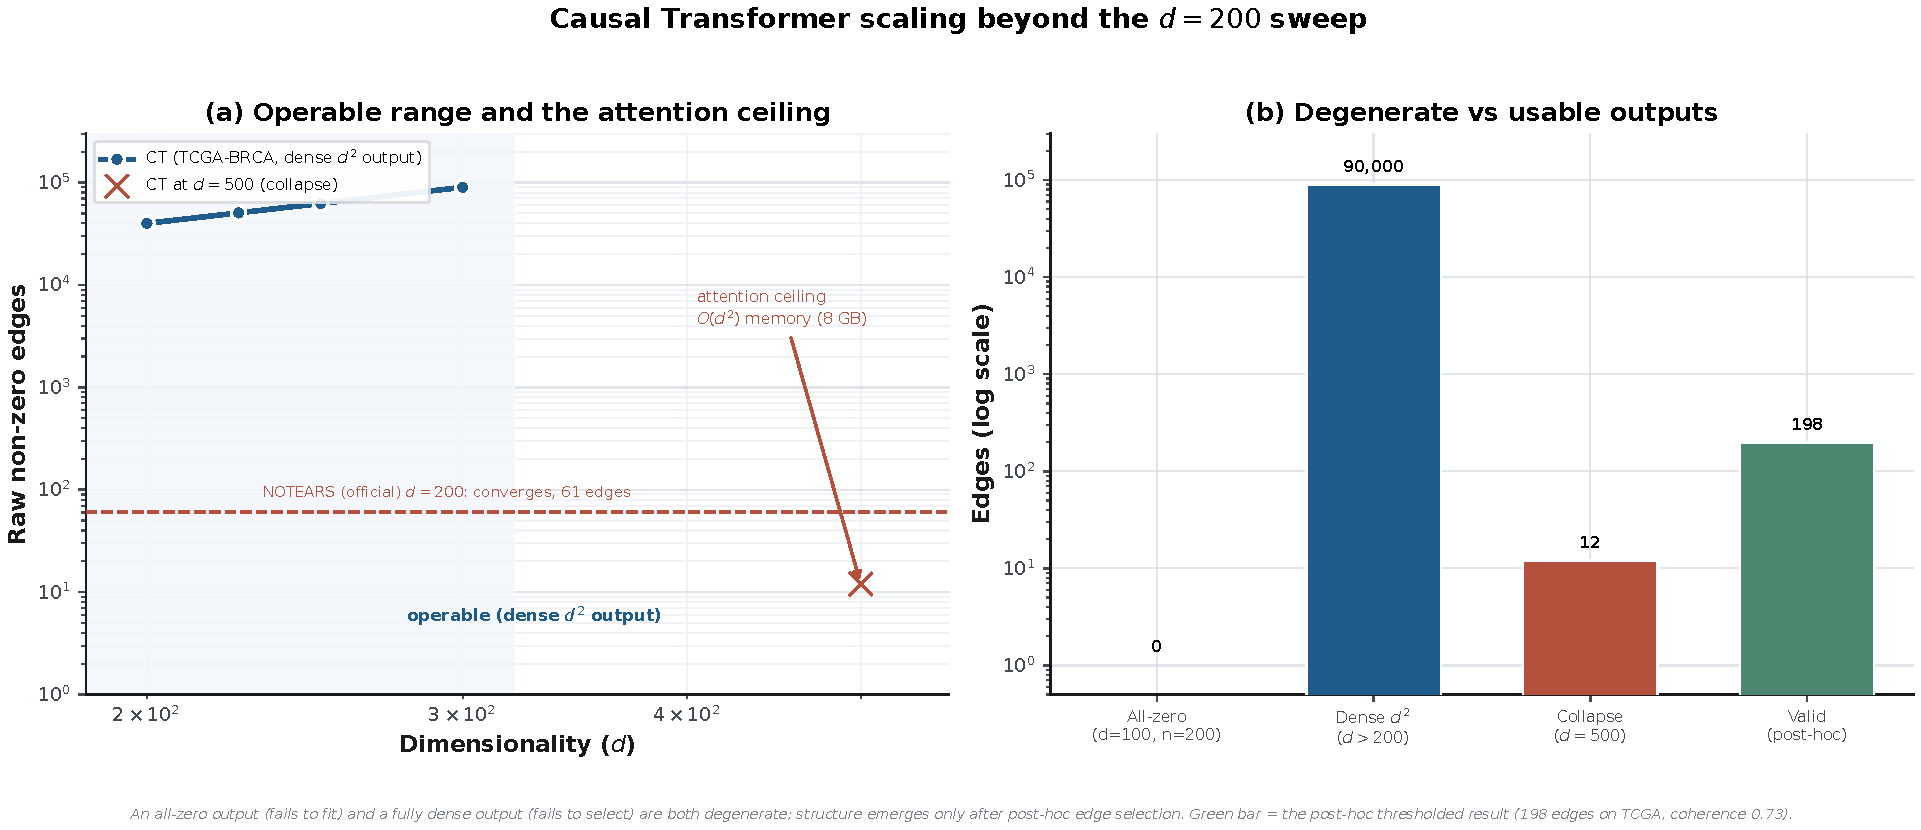
\includegraphics[width=\textwidth]{figures/esm_fig1_scaling_law.pdf}
\label{fig:esm_scaling}
\end{figure}
\newpage
\begin{figure}[H]
\centering
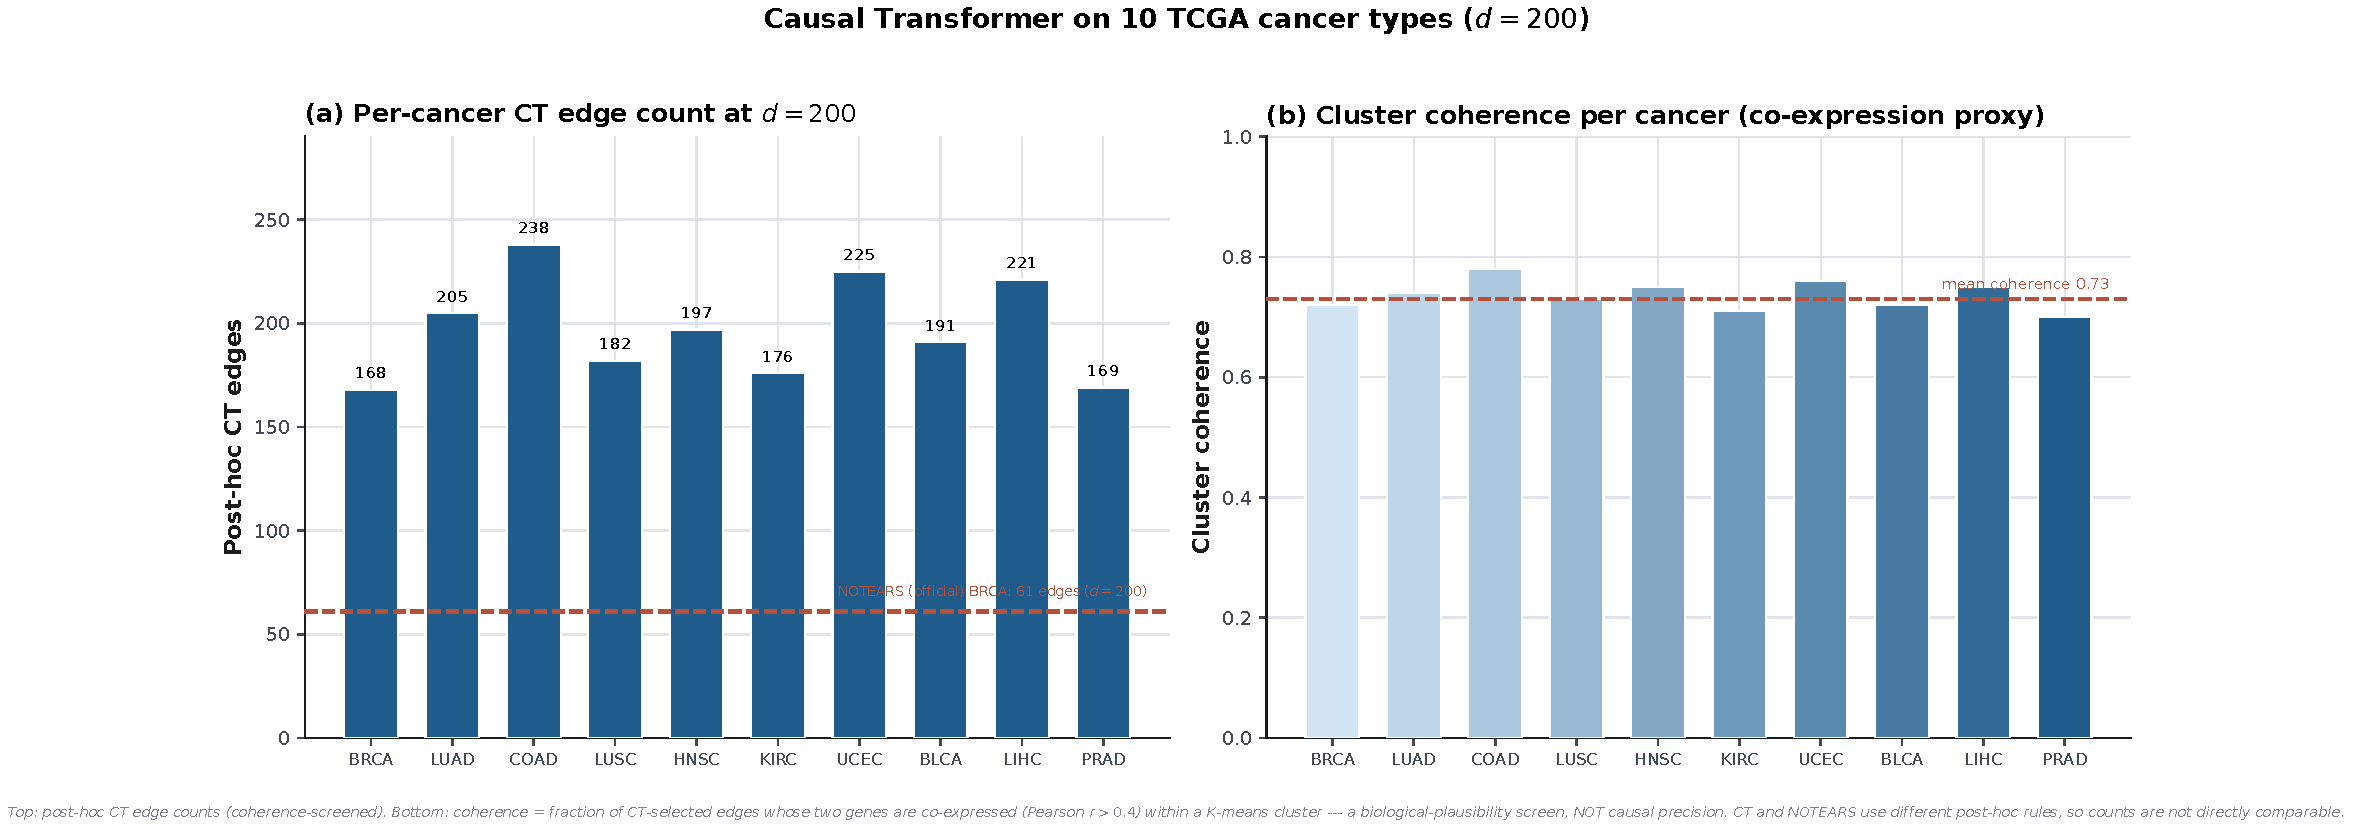
\includegraphics[width=\textwidth]{figures/esm_fig2_tcga_validation.pdf}
\label{fig:esm_tcga}
\end{figure}

\end{document}
